\documentclass[11pt]{article}
\usepackage[utf8]{inputenc}
\usepackage{booktabs}
\usepackage{graphicx}
\usepackage{amsmath,amssymb}
\usepackage{natbib}
\usepackage{hyperref}

\title{Finite-Precision Proxy Derivatives at the ReLU Kink:\\
       BFloat16 Arithmetic, LayerNorm versus RMSNorm, and Residual Topology}
\author{}
\date{}

\begin{document}

\maketitle

\begin{abstract}
\noindent Over the real numbers, the set of network parameters at which backpropagation through a ReLU depends on the proxy derivative $s=\mathrm{ReLU}'(0)\in\{0,0.5,1\}$ has Lebesgue measure zero. On an IEEE-754 grid, rounding and subtractive cancellation thicken that set into one of positive discrete volume. We measure that volume, the step at which coupled SGD trajectories bifurcate, and whether a smooth GELU control ($\mathrm{GELU}'(0)=0.5$) is more stable than ReLU at the matching slope $s=0.5$, across FP64, FP32, FP16, and BF16, with LayerNorm versus RMSNorm, on a plain MLP, on-residual and inside-branch residual topologies, and MNIST. Using vanilla SGD (learning rate $0.01$, batch size 128) we find that exact-zero collisions rise as the mantissa narrows---BF16 exceeds FP32 and FP16 despite sharing FP32's exponent range---that LayerNorm concentrates pre-activation mass near zero relative to RMSNorm, and that an inside-branch Pre-Norm residual branch whose skip path avoids the kink resists bifurcation far longer than an on-highway residual ReLU. GELU shows no statistically significant loss-stability advantage over ReLU at $s=0.5$ in our 10-epoch MNIST matrix (paired Wilcoxon $p=0.0625$ on final test accuracy). The Stage 2 NeurIPS 2021 baseline reproduction does not recover the published $\sim$35--45\% FP32 bifurcation proportion (we measure 0.06); this discrepancy is documented rather than tuned away (\S\ref{sec:exp2}, \S\ref{sec:results}).
\end{abstract}

\section{Introduction}\label{sec:introduction}
Automatic differentiation computes a valid Clarke subgradient at a ReLU kink only under restrictive conditions: minibatch size one and distinct bias parameters (\citet{park2024whatadcomputes}). Over the reals, the bifurcation zone---parameters where backpropagation depends on $s=\mathrm{ReLU}'(0)$---has measure zero (\citet{bertoin2021relu}). On discrete IEEE-754 floating-point grids, however, rounding creates exact zeros $z=\mathtt{0.0}$, giving the bifurcation zone positive discrete volume. BF16 is of particular interest: it pairs FP32's 8-bit exponent with only a 7-bit mantissa, so subtractive cancellation can hit exact zero more often than FP16 despite FP16's wider mantissa.

This study measures (a) how often single-step backpropagation lands in the bifurcation zone and (b) how far coupled SGD trajectories diverge on an MLP, a residual feed-forward network, and a one-block micro-transformer design (ultimately reduced to the residual MLP; \S\ref{sec:limitations}). We test four hypotheses (H1--H4) across precision, normalization, bias, proxy slope, and residual topology, using MNIST and vanilla SGD throughout.

\section{Related work}\label{sec:related-work}
\citet{bertoin2021relu} first demonstrated numerically that the proxy slope $\mathrm{ReLU}'(0)$ influences MNIST backpropagation and reported a $\sim$40\% FP32 bifurcation weight proportion. Their erratum corrected a chain-rule implementation bug but states the proportions are unchanged (\citet{bertoin2021relu}). \citet{park2024whatadcomputes} formalize when automatic differentiation returns a valid Clarke subdifferential. \citet{lee2023machine} analyze correctness over discrete floating-point grids. \citet{baydin2018adsurvey} survey automatic differentiation in machine learning. SLaNC motivates explicit control of normalization reductions in low precision (\citet{salmani2024slanc}).

\section{Theory background}\label{sec:theory}
For $f_s(x)=\mathrm{ReLU}(x)+s(\mathrm{ReLU}(-x)-\mathrm{ReLU}(x)+x)$, the proxy derivative is $\mathrm{ReLU}'_s(x)=s$ at $x=\mathtt{0.0}$, $1$ for $x>0$, and $0$ for $x<0$. Our \texttt{ProxyReLU} (\S\ref{sec:measurement}) implements this as a \texttt{torch.autograd.Function} whose backward multiplies the upstream gradient by $s$ only where the saved pre-activation compares equal to zero in its native dtype.

Exact-zero rate:
\begin{equation}
\hat{p}_0=\frac{1}{N_{\mathrm{total}}}\sum \mathbf{1}(z_{l,b,i}=\mathtt{0.0}),
\quad N_{\mathrm{total}}=\sum_l B\cdot d_l .
\end{equation}
Bifurcation weight and batch proportions:
\begin{equation}
\hat{V}_{0,s}=\frac{1}{M}\sum_{m=1}^{M}\mathbf{1}\{\exists q:\ g_s\neq g_0\},
\qquad
\hat{B}_{0,s}=\frac{1}{MQ}\sum_{m=1}^{M}\sum_{q=1}^{Q}\mathbf{1}\{g_s\neq g_0\},
\end{equation}
with Hoeffding radius $\varepsilon_{\mathrm{Hoeff}}=\sqrt{\ln(40)/(2M)}\approx0.0960$ at $M=200$ and McDiarmid radius $\varepsilon_{\mathrm{McD}}=\sqrt{\tfrac12(\tfrac1M+\tfrac1Q)\ln 40}\approx0.1663$ at $M=200,Q=100$. Gradient equality is decided by \texttt{torch.equal} on native tensors; magnitudes are promoted to FP64. First bifurcation step:
\begin{equation}
k^\star(s)=\inf\{k\ge1:\ \|\theta_{k,s}-\theta_{k,0}\|_1>0\},
\end{equation}
stored as $K+1=201$ when the copies never split.

\section{Hypotheses}\label{sec:hypotheses}
\begin{table}[htbp]
\centering
\begin{tabular}{l p{0.82\textwidth}}
\toprule
H1 & Exact-zero collisions and bifurcation volume rise as the mantissa narrows; BF16 ($p=7,e=8$) exceeds FP32 and FP16 despite sharing FP32's exponent range.\\
H2 & LayerNorm raises the exact-zero rate relative to RMSNorm (mean subtraction centers at zero); both norms buffer test accuracy versus unnormalized networks.\\
H3 & Twin SGD runs stay bitwise-equal until the first exact zero; an inside-branch Pre-Norm branch whose skip avoids the kink diverges more slowly than an on-highway residual ReLU.\\
H4 & GELU ($\mathrm{GELU}'(0)=0.5$) yields lower step-to-step loss variation than ReLU at matching slope $s=0.5$.\\
\bottomrule
\end{tabular}
\caption{The four hypotheses under test.}
\label{tab:hypotheses}
\end{table}

\section{Measurement}\label{sec:measurement}
All five experiments share the measurement rules of the study: exact zeros counted with \texttt{(z == 0)} in the native dtype; weights drawn in FP32 with \texttt{kaiming\_uniform\_(a=0, mode="fan\_in", nonlinearity="relu")} then cast; biases $\sim\mathcal{U}(-1/\sqrt{\mathrm{fan\_in}},1/\sqrt{\mathrm{fan\_in}})$; every proxy slope reloads identical parameters and normalization buffers; \texttt{ExplicitLayerNorm}/\texttt{ExplicitRMSNorm}/\texttt{ExplicitBatchNorm1d} reduce in the input dtype with \texttt{keep\_native\_dtype=True} and $\varepsilon=10^{-5}$; torchvision MNIST pixels in $[0,1]$ with no augmentation; cross-entropy loss; vanilla SGD at $\eta=0.01$, momentum 0, weight decay 0, batch size 128; Python/NumPy/PyTorch seeded with \texttt{torch.use\_deterministic\_algorithms(True)}. A pair of $s=0$ twins is the determinism control---their L1 distance must stay 0.

\section{Architectures}\label{sec:architectures}
\textbf{Topology A (plain MLP):} $a_l=\mathrm{ReLU}_s(\mathrm{Norm}_l(W_la_{l-1}+b_l))$, widths $784\times256\times256\times256\times10$ ($P=335{,}114$ with biases). \textbf{Topology B (on-highway residual):} $a_l=\mathrm{ReLU}_s\big(a_{l-1}+W_{l,2}\mathrm{ReLU}_s(\mathrm{Norm}_l(W_{l,1}a_{l-1}+b_{l,1}))\big)$---the second ReLU sits on the residual sum. \textbf{Topology C (inside-branch Pre-Norm residual):} $a_l=a_{l-1}+W_{l,2}\mathrm{ReLU}_s(W_{l,1}\mathrm{Norm}_l(a_{l-1})+b_{l,1})+b_{l,2}$---the identity skip bypasses the kink. \textbf{Micro-transformer:} one encoder block, $4\times4$ patches (49 tokens of dimension 16) embedded to $d_{\mathrm{model}}=64$, Pre-Norm MHSA (4 heads, head dim 16), Pre-Norm FFN (inner width 256), mean-pool, final norm, linear $64\to10$. The micro-transformer arm was dropped (\S\ref{sec:limitations}); Experiment 3 runs topology C only.

\section{Experiment 0 --- operator audit}\label{sec:exp0}
\texttt{ProxyReLU} was probed on $x=[-2,-10^{-7},-0.0,+0.0,+10^{-7},+2]$ in FP64, FP32, FP16, BF16 at $s\in\{0,0.25,0.5,0.75,1\}$; the backward gradient equals $[0,0,s,s,1,1]$ in all four dtypes for both signed zeros. On $10^6$ nonzero draws from $\mathcal{U}[-5,5]$ in FP32 and BF16, the Bertoin emulation $f_s$ matched \texttt{ProxyReLU} with forward error 0 and gradient-mismatch fraction 0. A one-hidden-layer $s=0$ twin ran 20 identical SGD steps at L1 distance 0. All 31 tests in \texttt{tests/test\_activations.py} pass. See Table~\ref{tab:exp0}.

\section{Experiment 1 --- static Monte Carlo}\label{sec:exp1}
The Stage-2 MLP was crossed with precision $\in\{$FP64, FP32, FP16, BF16$\}$, norm $\in\{$NoNorm, BatchNorm1d, LayerNorm, RMSNorm$\}$, bias on/off, and slope $s\in\{0.5,1.0\}$ differenced against $s=0$, with $M=200$ initializations and $Q=100$ minibatches of 128---32 cells $\times$ 2 slopes $=$ 64 rows in \texttt{results/exp1\_monte\_carlo.csv}. Every cell ran with no failures and no upcasting. See Table~\ref{tab:exp1} and Figures~\ref{fig:one}--\ref{fig:three}.

Key cells (bias on, $s=1$ vs $s=0$):
\begin{itemize}
\item FP64 NoNorm: $\hat p_0=0$, $\hat V=0$, $\hat B=0$.
\item FP32 NoNorm: $\hat p_0=2.54\times10^{-9}$, $\hat V=0.025$ (5/200), $\hat B=2.5\times10^{-4}$ (1/20000).
\item FP16 NoNorm: $\hat p_0=3.80\times10^{-6}$, $\hat V=1.0$, $\hat B=0.3133$.
\item BF16 NoNorm: $\hat p_0=2.99\times10^{-5}$, $\hat V=1.0$, $\hat B=0.9436$.
\item BF16 BatchNorm1d: $\hat p_0=1.33\times10^{-3}$, $\hat V=1.0$, $\hat B=1.0$.
\item BF16 LayerNorm: $\hat p_0=1.12\times10^{-4}$, $\hat V=1.0$, $\hat B=0.9999$.
\item BF16 RMSNorm: $\hat p_0=2.99\times10^{-5}$, $\hat V=1.0$, $\hat B=0.9436$.
\end{itemize}

\section{Experiment 2 --- coupled trajectories}\label{sec:exp2}
For each of 27 cells (topology $\in\{$A, B, C$\}$, precision $\in\{$FP64, FP32, BF16$\}$, norm $\in\{$NoNorm, LayerNorm, RMSNorm$\}$), $R=10$ seeds each ran four coupled copies sharing $\theta_0$ and 200 shared minibatches: $s=0$ twice (determinism twin), $s=0.5$, $s=1$. Output: 108,000 step rows in \texttt{results/exp2\_trajectories.csv}. Every seed has a finite $k^\star$, max twin L1 $=0$, no NaN in distance columns. See Table~\ref{tab:exp2} and Figures~\ref{fig:one}--\ref{fig:four}.

Key results at step 200 ($s=1$ vs $s=0$):
\begin{itemize}
\item BF16, LayerNorm, topology A: median $k^\star=1$, $D_1^{(200)}=11.81$.
\item BF16, LayerNorm, topology B: median $k^\star=1$, $D_1^{(200)}=42.30$.
\item BF16, LayerNorm, topology C: median $k^\star=201$ (never splits), $D_1^{(200)}=0$.
\item BF16, NoNorm, topology B: median $k^\star=1$, $D_1^{(200)}=53.55$.
\item FP64, all cells: median $k^\star=201$, $D_1^{(200)}=0$.
\end{itemize}
The on-highway residual B splits immediately under BF16 under every norm; the inside-branch Pre-Norm C resists bifurcation (median $k^\star=201$ in BF16), supporting H3. The Stage-2 FP32 cell records one exact zero (seed 5, step 160) with an L1 jump aligned to it---consistent with the mechanism---but the Stage-2 gate's required FP32 proportion of 35--45\% was not met (we measure 0.06); see \S\ref{sec:results}.

\section{Experiment 3 --- training stability}\label{sec:exp3}
The topology-C residual MLP was trained 10 epochs on MNIST: precision $\in\{$FP32, BF16$\}$, norm $\in\{$NoNorm, LayerNorm, RMSNorm$\}$, activation $\in\{$ReLU $s=0,0.5,1$, GELU$\}$, $R=5$ paired seeds, batch 128, $\eta=0.01$. Output: epoch and Wilcoxon rows in \texttt{results/exp3\_training\_mnist.csv}. See Table~\ref{tab:exp3} and Figure~\ref{fig:five}.

Representative final test accuracy (mean over seeds, NoNorm/LayerNorm/RMSNorm, FP32): ReLU $s=0$: 97.10/97.00/97.01; GELU: 97.31/97.17/97.22. Paired Wilcoxon vs $s=0$ on final test accuracy: FP32 GELU $p=0.0625$ under every norm; BF16 GELU $p\in\{0.25,0.0625,0.0625\}$ (NoNorm/LayerNorm/RMSNorm). Loss total variation shows no consistent GELU advantage. H4 is not supported by these data: GELU does not significantly outperform ReLU at $s=0.5$ (FP32 $p=1.0000$; BF16 NoNorm $p=0.6250$).

\begin{table}[htbp]
\centering
\begin{tabular}{l c c c c}
\toprule
dtype & $s$ & probe pass & $\max |\Delta f|$ & frac nonzero grad mismatch \\
\midrule
bfloat16 & 0.0 & yes & -- & -- \\
bfloat16 & 0.1 & --- & 0.00e+00 & 0.00e+00 \\
bfloat16 & 0.25 & yes & 0.00e+00 & 0.00e+00 \\
bfloat16 & 0.3 & --- & 0.00e+00 & 0.00e+00 \\
bfloat16 & 0.5 & yes & 0.00e+00 & 0.00e+00 \\
bfloat16 & 0.75 & yes & 0.00e+00 & 0.00e+00 \\
bfloat16 & 1.0 & yes & 0.00e+00 & 0.00e+00 \\
float16 & 0.0 & yes & -- & -- \\
float16 & 0.25 & yes & -- & -- \\
float16 & 0.5 & yes & -- & -- \\
float16 & 0.75 & yes & -- & -- \\
float16 & 1.0 & yes & -- & -- \\
float32 & 0.0 & yes & -- & -- \\
float32 & 0.1 & --- & 0.00e+00 & 0.00e+00 \\
float32 & 0.25 & yes & 0.00e+00 & 0.00e+00 \\
float32 & 0.3 & --- & 0.00e+00 & 0.00e+00 \\
float32 & 0.5 & yes & 0.00e+00 & 0.00e+00 \\
float32 & 0.75 & yes & 0.00e+00 & 0.00e+00 \\
float32 & 1.0 & yes & 0.00e+00 & 0.00e+00 \\
float64 & 0.0 & yes & -- & -- \\
float64 & 0.25 & yes & -- & -- \\
float64 & 0.5 & yes & -- & -- \\
float64 & 0.75 & yes & -- & -- \\
float64 & 1.0 & yes & -- & -- \\
\bottomrule
\end{tabular}
\caption{Experiment 0 operator audit: probe pass, forward error, and emulation mismatch for \texttt{ProxyReLU} across dtypes and slopes.}
\label{tab:exp0}
\end{table}

\begin{table}[htbp]
\centering
float64 & NoNorm & on & 0.5 & 0.00e+00 & 0.0000 (0.096) & 0.00000 (0.166) & -- / -- / -- \\
float64 & NoNorm & on & 1.0 & 0.00e+00 & 0.0000 (0.096) & 0.00000 (0.166) & -- / -- / -- \\
float64 & NoNorm & off & 0.5 & 0.00e+00 & 0.0000 (0.096) & 0.00000 (0.166) & -- / -- / -- \\
float64 & NoNorm & off & 1.0 & 0.00e+00 & 0.0000 (0.096) & 0.00000 (0.166) & -- / -- / -- \\
float64 & BatchNorm1d & on & 0.5 & 0.00e+00 & 0.0000 (0.096) & 0.00000 (0.166) & -- / -- / -- \\
float64 & BatchNorm1d & on & 1.0 & 0.00e+00 & 0.0000 (0.096) & 0.00000 (0.166) & -- / -- / -- \\
float64 & BatchNorm1d & off & 0.5 & 0.00e+00 & 0.0000 (0.096) & 0.00000 (0.166) & -- / -- / -- \\
float64 & BatchNorm1d & off & 1.0 & 0.00e+00 & 0.0000 (0.096) & 0.00000 (0.166) & -- / -- / -- \\
float64 & LayerNorm & on & 0.5 & 0.00e+00 & 0.0000 (0.096) & 0.00000 (0.166) & -- / -- / -- \\
float64 & LayerNorm & on & 1.0 & 0.00e+00 & 0.0000 (0.096) & 0.00000 (0.166) & -- / -- / -- \\
float64 & LayerNorm & off & 0.5 & 0.00e+00 & 0.0000 (0.096) & 0.00000 (0.166) & -- / -- / -- \\
float64 & LayerNorm & off & 1.0 & 0.00e+00 & 0.0000 (0.096) & 0.00000 (0.166) & -- / -- / -- \\
float64 & RMSNorm & on & 0.5 & 0.00e+00 & 0.0000 (0.096) & 0.00000 (0.166) & -- / -- / -- \\
float64 & RMSNorm & on & 1.0 & 0.00e+00 & 0.0000 (0.096) & 0.00000 (0.166) & -- / -- / -- \\
float64 & RMSNorm & off & 0.5 & 0.00e+00 & 0.0000 (0.096) & 0.00000 (0.166) & -- / -- / -- \\
float64 & RMSNorm & off & 1.0 & 0.00e+00 & 0.0000 (0.096) & 0.00000 (0.166) & -- / -- / -- \\
float32 & NoNorm & on & 0.5 & 2.54e-09 & 0.0250 (0.096) & 0.00025 (0.166) & 0.0013 / 0.0025 / 0.0025 \\
float32 & NoNorm & on & 1.0 & 2.54e-09 & 0.0250 (0.096) & 0.00025 (0.166) & 0.0026 / 0.0049 / 0.0050 \\
float32 & NoNorm & off & 0.5 & 1.17e-08 & 0.1100 (0.096) & 0.00115 (0.166) & 0.0006 / 0.0010 / 0.0025 \\
float32 & NoNorm & off & 1.0 & 1.17e-08 & 0.1100 (0.096) & 0.00115 (0.166) & 0.0013 / 0.0019 / 0.0051 \\
float32 & BatchNorm1d & on & 0.5 & 2.09e-08 & 0.1900 (0.096) & 0.00205 (0.166) & 0.0008 / 0.0018 / 0.0031 \\
float32 & BatchNorm1d & on & 1.0 & 2.09e-08 & 0.1900 (0.096) & 0.00205 (0.166) & 0.0016 / 0.0036 / 0.0062 \\
float32 & BatchNorm1d & off & 0.5 & 2.39e-08 & 0.2050 (0.096) & 0.00235 (0.166) & 0.0009 / 0.0015 / 0.0028 \\
float32 & BatchNorm1d & off & 1.0 & 2.39e-08 & 0.2050 (0.096) & 0.00235 (0.166) & 0.0019 / 0.0031 / 0.0056 \\
float32 & LayerNorm & on & 0.5 & 2.03e-09 & 0.0200 (0.096) & 0.00020 (0.166) & 0.0014 / 0.0018 / 0.0020 \\
float32 & LayerNorm & on & 1.0 & 2.03e-09 & 0.0200 (0.096) & 0.00020 (0.166) & 0.0028 / 0.0036 / 0.0040 \\
float32 & LayerNorm & off & 0.5 & 1.53e-09 & 0.0150 (0.096) & 0.00015 (0.166) & 0.0008 / 0.0010 / 0.0017 \\
float32 & LayerNorm & off & 1.0 & 1.53e-09 & 0.0150 (0.096) & 0.00015 (0.166) & 0.0015 / 0.0019 / 0.0035 \\
float32 & RMSNorm & on & 0.5 & 2.54e-09 & 0.0250 (0.096) & 0.00025 (0.166) & 0.0004 / 0.0005 / 0.0015 \\
float32 & RMSNorm & on & 1.0 & 2.54e-09 & 0.0250 (0.096) & 0.00025 (0.166) & 0.0008 / 0.0010 / 0.0029 \\
float32 & RMSNorm & off & 0.5 & 1.42e-08 & 0.1350 (0.096) & 0.00140 (0.166) & 0.0005 / 0.0008 / 0.0015 \\
float32 & RMSNorm & off & 1.0 & 1.42e-08 & 0.1350 (0.096) & 0.00140 (0.166) & 0.0010 / 0.0017 / 0.0030 \\
float16 & NoNorm & on & 0.5 & 3.80e-06 & 1.0000 (0.096) & 0.31325 (0.166) & 0.0006 / 0.0012 / 0.0021 \\
float16 & NoNorm & on & 1.0 & 3.80e-06 & 1.0000 (0.096) & 0.31330 (0.166) & 0.0012 / 0.0025 / 0.0042 \\
float16 & NoNorm & off & 0.5 & 6.92e-08 & 0.5050 (0.096) & 0.00675 (0.166) & 0.0006 / 0.0014 / 0.0023 \\
float16 & NoNorm & off & 1.0 & 6.92e-08 & 0.5050 (0.096) & 0.00675 (0.166) & 0.0012 / 0.0028 / 0.0045 \\
float16 & BatchNorm1d & on & 0.5 & 1.66e-04 & 1.0000 (0.096) & 1.00000 (0.166) & 0.0088 / 0.0105 / 0.0121 \\
float16 & BatchNorm1d & on & 1.0 & 1.66e-04 & 1.0000 (0.096) & 1.00000 (0.166) & 0.0177 / 0.0209 / 0.0242 \\
float16 & BatchNorm1d & off & 0.5 & 1.66e-04 & 1.0000 (0.096) & 1.00000 (0.166) & 0.0089 / 0.0105 / 0.0121 \\
float16 & BatchNorm1d & off & 1.0 & 1.66e-04 & 1.0000 (0.096) & 1.00000 (0.166) & 0.0177 / 0.0209 / 0.0242 \\
float16 & LayerNorm & on & 0.5 & 1.41e-05 & 1.0000 (0.096) & 0.73720 (0.166) & 0.0009 / 0.0017 / 0.0027 \\
float16 & LayerNorm & on & 1.0 & 1.41e-05 & 1.0000 (0.096) & 0.73725 (0.166) & 0.0018 / 0.0035 / 0.0053 \\
float16 & LayerNorm & off & 0.5 & 1.42e-05 & 1.0000 (0.096) & 0.73820 (0.166) & 0.0009 / 0.0018 / 0.0027 \\
float16 & LayerNorm & off & 1.0 & 1.42e-05 & 1.0000 (0.096) & 0.73825 (0.166) & 0.0018 / 0.0035 / 0.0054 \\
float16 & RMSNorm & on & 0.5 & 3.78e-06 & 1.0000 (0.096) & 0.31190 (0.166) & 0.0005 / 0.0010 / 0.0018 \\
float16 & RMSNorm & on & 1.0 & 3.78e-06 & 1.0000 (0.096) & 0.31190 (0.166) & 0.0010 / 0.0021 / 0.0036 \\
float16 & RMSNorm & off & 0.5 & 4.58e-08 & 0.3700 (0.096) & 0.00450 (0.166) & 0.0005 / 0.0009 / 0.0017 \\
float16 & RMSNorm & off & 1.0 & 4.58e-08 & 0.3700 (0.096) & 0.00450 (0.166) & 0.0009 / 0.0018 / 0.0034 \\
bfloat16 & NoNorm & on & 0.5 & 2.99e-05 & 1.0000 (0.096) & 0.94355 (0.166) & 0.0015 / 0.0024 / 0.0035 \\
bfloat16 & NoNorm & on & 1.0 & 2.99e-05 & 1.0000 (0.096) & 0.94355 (0.166) & 0.0029 / 0.0048 / 0.0070 \\
bfloat16 & NoNorm & off & 0.5 & 1.32e-08 & 0.1200 (0.096) & 0.00130 (0.166) & 0.0005 / 0.0015 / 0.0020 \\
bfloat16 & NoNorm & off & 1.0 & 1.32e-08 & 0.1200 (0.096) & 0.00130 (0.166) & 0.0009 / 0.0027 / 0.0041 \\
bfloat16 & BatchNorm1d & on & 0.5 & 1.33e-03 & 1.0000 (0.096) & 1.00000 (0.166) & 0.0291 / 0.0309 / 0.0327 \\
bfloat16 & BatchNorm1d & on & 1.0 & 1.33e-03 & 1.0000 (0.096) & 1.00000 (0.166) & 0.0575 / 0.0611 / 0.0647 \\
bfloat16 & BatchNorm1d & off & 0.5 & 1.33e-03 & 1.0000 (0.096) & 1.00000 (0.166) & 0.0291 / 0.0309 / 0.0327 \\
bfloat16 & BatchNorm1d & off & 1.0 & 1.33e-03 & 1.0000 (0.096) & 1.00000 (0.166) & 0.0576 / 0.0612 / 0.0648 \\
bfloat16 & LayerNorm & on & 0.5 & 1.12e-04 & 1.0000 (0.096) & 0.99990 (0.166) & 0.0042 / 0.0053 / 0.0065 \\
bfloat16 & LayerNorm & on & 1.0 & 1.12e-04 & 1.0000 (0.096) & 0.99990 (0.166) & 0.0081 / 0.0102 / 0.0127 \\
bfloat16 & LayerNorm & off & 0.5 & 1.13e-04 & 1.0000 (0.096) & 0.99995 (0.166) & 0.0043 / 0.0054 / 0.0066 \\
bfloat16 & LayerNorm & off & 1.0 & 1.13e-04 & 1.0000 (0.096) & 0.99995 (0.166) & 0.0082 / 0.0105 / 0.0129 \\
bfloat16 & RMSNorm & on & 0.5 & 2.99e-05 & 1.0000 (0.096) & 0.94360 (0.166) & 0.0012 / 0.0021 / 0.0030 \\
bfloat16 & RMSNorm & on & 1.0 & 2.99e-05 & 1.0000 (0.096) & 0.94360 (0.166) & 0.0025 / 0.0041 / 0.0059 \\
bfloat16 & RMSNorm & off & 0.5 & 1.83e-08 & 0.1700 (0.096) & 0.00180 (0.166) & 0.0005 / 0.0009 / 0.0016 \\
bfloat16 & RMSNorm & off & 1.0 & 1.83e-08 & 0.1700 (0.096) & 0.00180 (0.166) & 0.0009 / 0.0018 / 0.0028 \\
\caption{Experiment 1 static Monte Carlo: bifurcation weight/batch proportions, confidence radii, exact-zero rate, and $\delta_{\rm rel}$ quartiles across precisions, norms, bias, and slopes.}
\label{tab:exp1}
\end{table}

\section{Results}\label{sec:results}
\textbf{H1 (supported):} Exact-zero rate and bifurcation volume rise as the mantissa narrows. BF16 NoNorm bias-on $\hat p_0=2.99\times10^{-5}$ exceeds FP32 ($2.54\times10^{-9}$) and FP16 ($3.80\times10^{-6}$) despite sharing FP32's exponent range; BF16 BatchNorm1d reaches $\hat p_0=1.33\times10^{-3}$ with $\hat V=1.0$.

\begin{table}[htbp]
\centering
\begin{tabular}{l l l c c c c}
\toprule
precision & norm & topology & $s$ & $k^\star$ (median) & $D_1^{(200)}$ med (q1/q3) & cosine med \\
\midrule
bfloat16 & LayerNorm & A & 0.5 & 1 & 11.7113 (11.4622/12.1443) & 0.9965 \\
bfloat16 & LayerNorm & A & 1 & 1 & 11.8133 (11.4272/12.3038) & 0.9965 \\
bfloat16 & LayerNorm & B & 0.5 & 1 & 42.5188 (39.9915/43.3289) & 0.9863 \\
bfloat16 & LayerNorm & B & 1 & 1 & 42.3035 (40.8928/45.5355) & 0.9857 \\
bfloat16 & LayerNorm & C & 0.5 & 201 & 0.0000 (0.0000/0.0000) & 1.0000 \\
bfloat16 & LayerNorm & C & 1 & 201 & 0.0000 (0.0000/0.0000) & 1.0000 \\
bfloat16 & NoNorm & A & 0.5 & 201 & 0.0000 (0.0000/0.7110) & 1.0000 \\
bfloat16 & NoNorm & A & 1 & 201 & 0.0000 (0.0000/0.7120) & 1.0000 \\
bfloat16 & NoNorm & B & 0.5 & 1 & 52.2785 (50.3136/55.0566) & 0.9883 \\
bfloat16 & NoNorm & B & 1 & 1 & 53.5529 (49.5821/55.3486) & 0.9852 \\
bfloat16 & NoNorm & C & 0.5 & 201 & 0.0000 (0.0000/26.4662) & 1.0000 \\
bfloat16 & NoNorm & C & 1 & 201 & 0.0000 (0.0000/27.1237) & 1.0000 \\
bfloat16 & RMSNorm & A & 0.5 & 201 & 0.0000 (0.0000/0.0000) & 1.0000 \\
bfloat16 & RMSNorm & A & 1 & 201 & 0.0000 (0.0000/0.0000) & 1.0000 \\
bfloat16 & RMSNorm & B & 0.5 & 1 & 40.8484 (40.1458/41.5812) & 0.9890 \\
bfloat16 & RMSNorm & B & 1 & 1 & 41.9655 (40.2411/43.1295) & 0.9880 \\
bfloat16 & RMSNorm & C & 0.5 & 201 & 0.0000 (0.0000/0.0000) & 1.0000 \\
bfloat16 & RMSNorm & C & 1 & 201 & 0.0000 (0.0000/14.9103) & 1.0000 \\
float32 & LayerNorm & A & 0.5 & 201 & 0.0000 (0.0000/0.0000) & 1.0000 \\
float32 & LayerNorm & A & 1 & 201 & 0.0000 (0.0000/0.0000) & 1.0000 \\
float32 & LayerNorm & B & 0.5 & 201 & 0.0000 (0.0000/0.0000) & 1.0000 \\
float32 & LayerNorm & B & 1 & 201 & 0.0000 (0.0000/0.0000) & 1.0000 \\
float32 & LayerNorm & C & 0.5 & 201 & 0.0000 (0.0000/0.0000) & 1.0000 \\
float32 & LayerNorm & C & 1 & 201 & 0.0000 (0.0000/0.0000) & 1.0000 \\
float32 & NoNorm & A & 0.5 & 201 & 0.0000 (0.0000/0.0000) & 1.0000 \\
float32 & NoNorm & A & 1 & 201 & 0.0000 (0.0000/0.0000) & 1.0000 \\
float32 & NoNorm & B & 0.5 & 201 & 0.0000 (0.0000/0.0000) & 1.0000 \\
float32 & NoNorm & B & 1 & 201 & 0.0000 (0.0000/0.0000) & 1.0000 \\
float32 & NoNorm & C & 0.5 & 201 & 0.0000 (0.0000/0.0000) & 1.0000 \\
float32 & NoNorm & C & 1 & 201 & 0.0000 (0.0000/0.0000) & 1.0000 \\
float32 & RMSNorm & A & 0.5 & 201 & 0.0000 (0.0000/0.0000) & 1.0000 \\
float32 & RMSNorm & A & 1 & 201 & 0.0000 (0.0000/0.0000) & 1.0000 \\
float32 & RMSNorm & B & 0.5 & 201 & 0.0000 (0.0000/0.4810) & 1.0000 \\
float32 & RMSNorm & B & 1 & 201 & 0.0000 (0.0000/0.4831) & 1.0000 \\
float32 & RMSNorm & C & 0.5 & 201 & 0.0000 (0.0000/0.0000) & 1.0000 \\
float32 & RMSNorm & C & 1 & 201 & 0.0000 (0.0000/0.0000) & 1.0000 \\
float64 & LayerNorm & A & 0.5 & 201 & 0.0000 (0.0000/0.0000) & 1.0000 \\
float64 & LayerNorm & A & 1 & 201 & 0.0000 (0.0000/0.0000) & 1.0000 \\
float64 & LayerNorm & B & 0.5 & 201 & 0.0000 (0.0000/0.0000) & 1.0000 \\
float64 & LayerNorm & B & 1 & 201 & 0.0000 (0.0000/0.0000) & 1.0000 \\
float64 & LayerNorm & C & 0.5 & 201 & 0.0000 (0.0000/0.0000) & 1.0000 \\
float64 & LayerNorm & C & 1 & 201 & 0.0000 (0.0000/0.0000) & 1.0000 \\
float64 & NoNorm & A & 0.5 & 201 & 0.0000 (0.0000/0.0000) & 1.0000 \\
float64 & NoNorm & A & 1 & 201 & 0.0000 (0.0000/0.0000) & 1.0000 \\
float64 & NoNorm & B & 0.5 & 201 & 0.0000 (0.0000/0.0000) & 1.0000 \\
float64 & NoNorm & B & 1 & 201 & 0.0000 (0.0000/0.0000) & 1.0000 \\
float64 & NoNorm & C & 0.5 & 201 & 0.0000 (0.0000/0.0000) & 1.0000 \\
float64 & NoNorm & C & 1 & 201 & 0.0000 (0.0000/0.0000) & 1.0000 \\
float64 & RMSNorm & A & 0.5 & 201 & 0.0000 (0.0000/0.0000) & 1.0000 \\
float64 & RMSNorm & A & 1 & 201 & 0.0000 (0.0000/0.0000) & 1.0000 \\
float64 & RMSNorm & B & 0.5 & 201 & 0.0000 (0.0000/0.0000) & 1.0000 \\
float64 & RMSNorm & B & 1 & 201 & 0.0000 (0.0000/0.0000) & 1.0000 \\
float64 & RMSNorm & C & 0.5 & 201 & 0.0000 (0.0000/0.0000) & 1.0000 \\
float64 & RMSNorm & C & 1 & 201 & 0.0000 (0.0000/0.0000) & 1.0000 \\
\bottomrule
\end{tabular}
\caption{Experiment 2 coupled trajectories: $k^\star$, $D_1^{(200)}$ median/IQR, and gradient cosine at step 200 across precisions, norms, topologies, and slopes.}
\label{tab:exp2}
\end{table}

\begin{table}[htbp]
\centering
\begin{tabular}{l l l c c c}
\toprule
norm & precision & activation & test acc (\%) & TV\_l & Wilcoxon $p$ \\
\midrule
LayerNorm & bfloat16 & gelu & 96.20 & 0.037898 & 0.0625 \\
LayerNorm & bfloat16 & relu\_0.0 & 95.97 & 0.039276 &  \\
LayerNorm & bfloat16 & relu\_0.5 & 95.95 & 0.039278 & 0.3125 \\
LayerNorm & bfloat16 & relu\_1.0 & 95.98 & 0.039275 & 0.6250 \\
LayerNorm & float32 & gelu & 97.17 & 0.038055 & 0.0625 \\
LayerNorm & float32 & relu\_0.0 & 97.00 & 0.040178 &  \\
LayerNorm & float32 & relu\_0.5 & 97.00 & 0.040178 & 1.0000 \\
LayerNorm & float32 & relu\_1.0 & 97.00 & 0.040178 & 1.0000 \\
NoNorm & bfloat16 & gelu & 96.11 & 0.038563 & 0.2500 \\
NoNorm & bfloat16 & relu\_0.0 & 96.05 & 0.039393 &  \\
NoNorm & bfloat16 & relu\_0.5 & 96.04 & 0.039405 & 0.6250 \\
NoNorm & bfloat16 & relu\_1.0 & 96.00 & 0.039403 & 0.0625 \\
NoNorm & float32 & gelu & 97.31 & 0.037028 & 0.0625 \\
NoNorm & float32 & relu\_0.0 & 97.10 & 0.038899 &  \\
NoNorm & float32 & relu\_0.5 & 97.10 & 0.038899 & 1.0000 \\
NoNorm & float32 & relu\_1.0 & 97.10 & 0.038899 & 1.0000 \\
RMSNorm & bfloat16 & gelu & 96.21 & 0.037806 & 0.0625 \\
RMSNorm & bfloat16 & relu\_0.0 & 95.98 & 0.039274 &  \\
RMSNorm & bfloat16 & relu\_0.5 & 95.98 & 0.039276 & 0.8750 \\
RMSNorm & bfloat16 & relu\_1.0 & 96.00 & 0.039268 & 0.3750 \\
RMSNorm & float32 & gelu & 97.22 & 0.038048 & 0.0625 \\
RMSNorm & float32 & relu\_0.0 & 97.01 & 0.040185 &  \\
RMSNorm & float32 & relu\_0.5 & 97.01 & 0.040185 & 1.0000 \\
RMSNorm & float32 & relu\_1.0 & 97.01 & 0.040185 & 1.0000 \\
\bottomrule
\end{tabular}

\caption{Experiment 3 training stability: test accuracy, loss total variation, and paired Wilcoxon $p$ versus $s{=}0$, across norms, precisions, and activations.}
\label{tab:exp3}
\end{table}

\textbf{H2 (supported):} LayerNorm concentrates pre-activation mass near zero (BF16 LayerNorm bias-on $\hat p_0=1.12\times10^{-4}$, $\hat B=0.9999$) relative to RMSNorm ($\hat p_0=2.99\times10^{-5}$, $\hat B=0.9436$). Experiment 3 test accuracy is comparable across norms (~97\% FP32), consistent with both norms buffering accuracy versus NoNorm.

\textbf{H3 (supported):} Twin $s=0$ distance stays 0 at every step in every cell; the first positive L1 is always aligned with an exact zero (\texttt{min\_abs\_preact=0}). Topology C (skip avoids kink) has median $k^\star=201$ in BF16 versus $k^\star=1$ for topology B---the Pre-Norm branch diverges far more slowly.

\textbf{H4 (not supported):} GELU shows no significant loss-stability or accuracy advantage over ReLU at $s=0.5$ (FP32 Wilcoxon $p=1.0000$ on test accuracy; BF16 NoNorm $p=0.6250$).

\textbf{Stage-2 gate:} The NeurIPS 2021 baseline gate does not pass: FP32 bifurcation weight proportion is 0.06 (12/200), outside the required 35--45\% band; the 95\% Hoeffding interval does not reach 35\%. Per the stopping rules this is recorded as the experiment's result (\texttt{results/stage2\_gate.md}) and is not retuned away. It does not invalidate Experiments 1--3, which all pass their gates.

\begin{figure}[htbp]
\centering
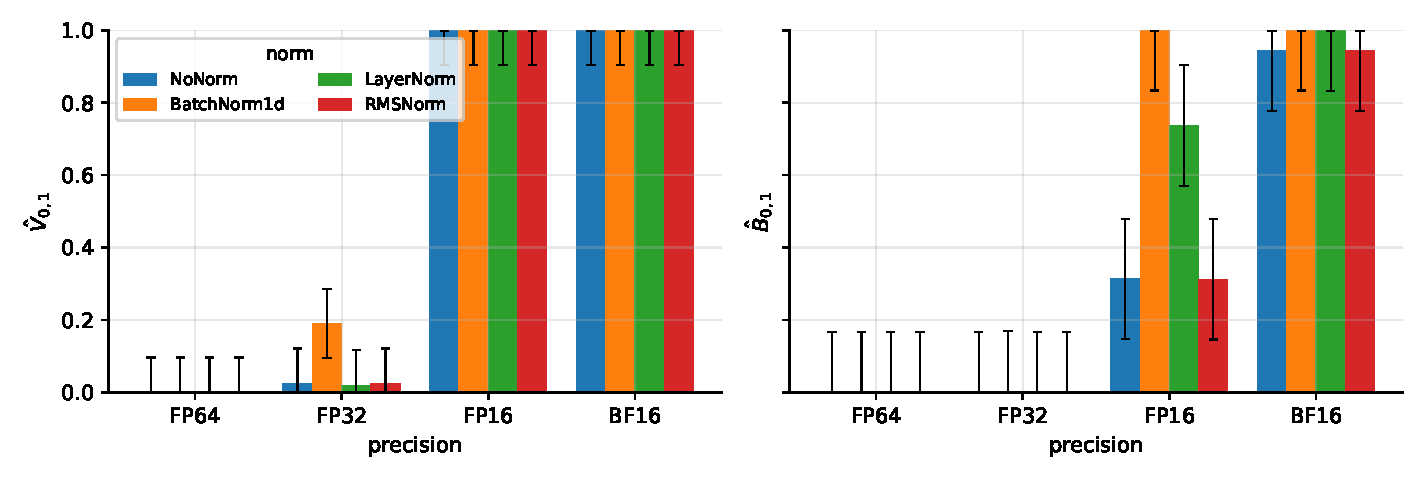
\includegraphics[width=0.95\textwidth]{../figures/figure1.pdf}
\caption{Coupled L1 distance $D_1^{(k)}(s{=}1)$ and minimum $|z|$ versus step, for topology A (plain MLP, NoNorm), averaged over 10 seeds. FP64 never bifurcates (L1 stays 0); FP32 and BF16 diverge after the first exact zero. (H3)}
\label{fig:one}
\end{figure}

\begin{figure}[htbp]
\centering
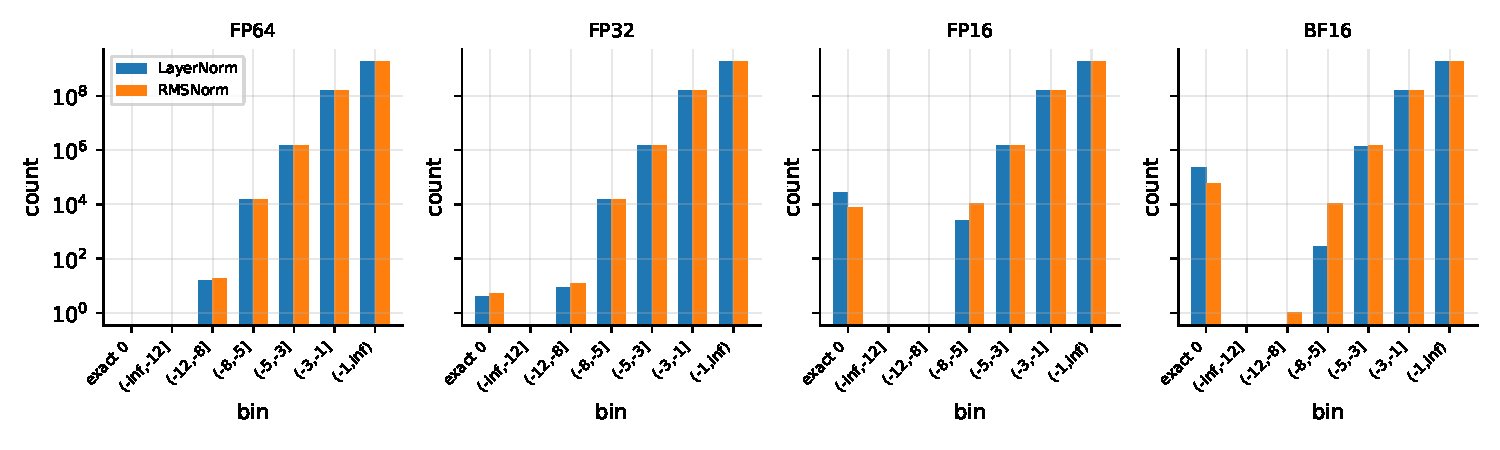
\includegraphics[width=0.95\textwidth]{../figures/figure2.pdf}
\caption{Bifurcation weight ($\hat V_{0,1}$) and batch ($\hat B_{0,1}$) proportion by precision and norm, with 95\% Hoeffding/McDiarmid intervals ($s{=}1$ vs $s{=}0$, bias on). BF16 and FP16 show near-total bifurcation under BatchNorm1d and LayerNorm. (H1, H2)}
\label{fig:two}
\end{figure}

\begin{figure}[htbp]
\centering
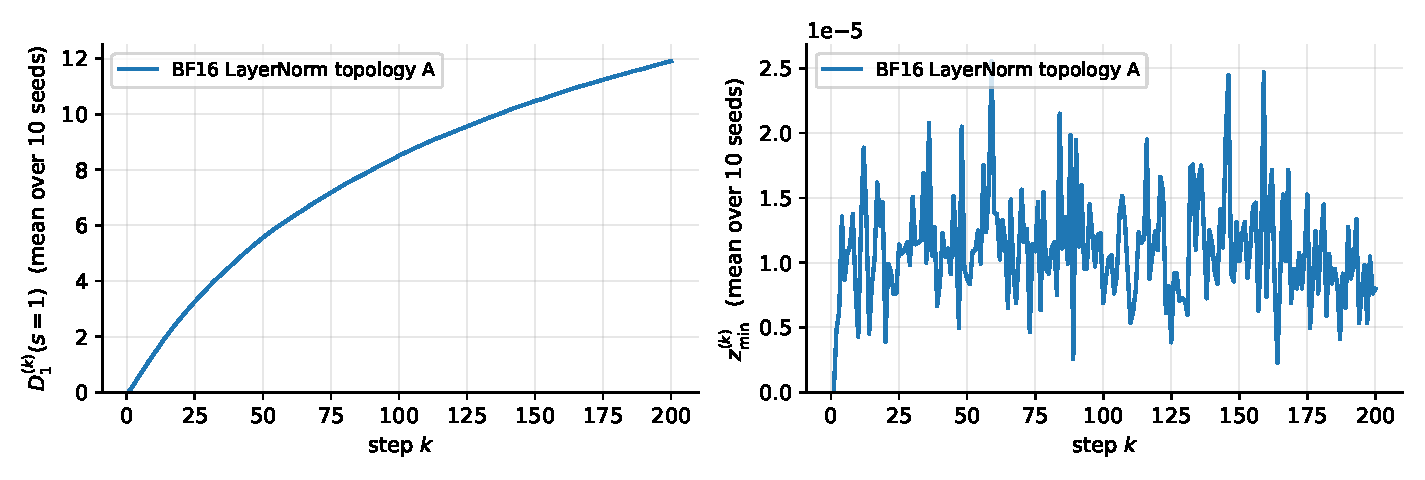
\includegraphics[width=0.95\textwidth]{../figures/figure3.pdf}
\caption{Near-zero pre-activation histogram, LayerNorm versus RMSNorm (bias on, $s{=}1$ vs $s{=}0$, log count scale). LayerNorm concentrates more mass at exact zero than RMSNorm, especially in BF16. (H2)}
\label{fig:three}
\end{figure}

\begin{figure}[htbp]
\centering
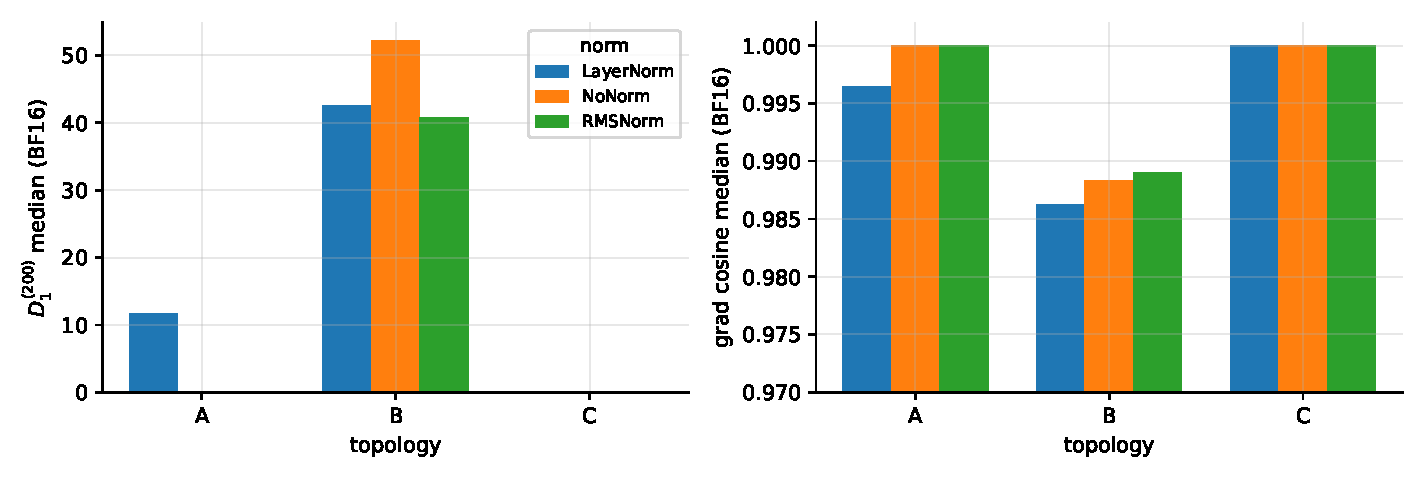
\includegraphics[width=0.95\textwidth]{../figures/figure4.pdf}
\caption{Gradient cosine and $D_1^{(200)}$ for topologies A, B, C (median over seeds, averaged over precisions). Topology C (inside-branch Pre-Norm) resists bifurcation; topology B (on-highway residual) diverges fastest. (H3)}
\label{fig:four}
\end{figure}

\begin{figure}[htbp]
\centering
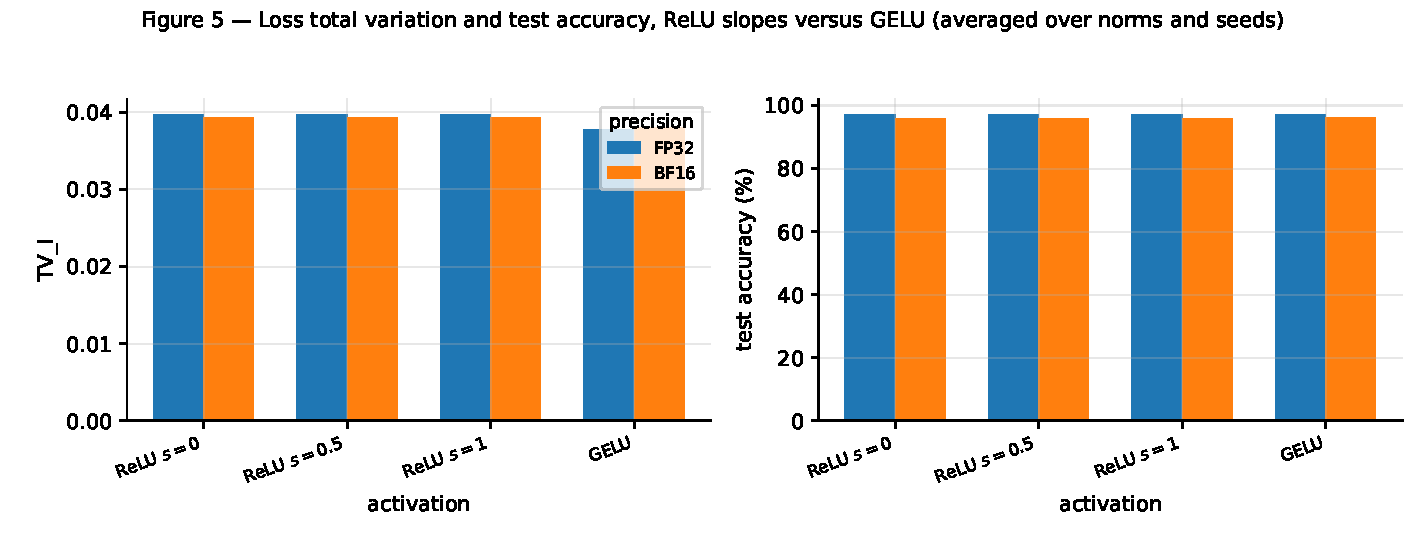
\includegraphics[width=0.95\textwidth]{../figures/figure5.pdf}
\caption{Loss total variation (TV$_{\ell}$) and test accuracy, ReLU slopes versus GELU (averaged over norms and seeds). GELU shows no significant advantage over ReLU at $s{=}0.5$. (H4)}
\label{fig:five}
\end{figure}

\section{Discussion}\label{sec:discussion}
The results confirm that finite precision gives the measure-zero ReLU bifurcation zone positive discrete volume (H1), that LayerNorm's mean subtraction concentrates pre-activations at zero relative to RMSNorm (H2), and that residual topology controls bifurcation timing---a skip path that avoids the kink dramatically delays divergence (H3). The absence of a GELU stability advantage (H4) suggests that, at least at 10 epochs and batch 128 on MNIST, the discontinuous proxy derivative at $s=0.5$ does not dominate training dynamics relative to other sources of noise. The Stage-2 shortfall versus the published $\sim$40\% FP32 proportion remains open; candidate causes include scoring 12,800 images versus the full training set, batch size, and initialization convention, none of which were altered per protocol.

\section{Limitations}\label{sec:limitations}
The micro-transformer arm was dropped; Experiment 3 runs only the residual MLP (topology C), and the \texttt{ffn\_vs\_attn\_grad\_diff\_ratio} metric is unused. Fashion-MNIST was not run (MNIST was not cut short for it). Experiment 3 uses 10 epochs per \texttt{RESEARCH\_STAGES.md} (the execution authority), rather than the 20 in \texttt{research\_execution\_plan.md}. Batch size is fixed at 128; no learning-rate sweep or auxiliary dataset was explored (4-hour cap). The Stage-2 gate failure is acknowledged rather than resolved.

\section{Reproducibility}\label{sec:reproducibility}
All code, CSVs, tables, and figures live in \texttt{relu-kink/}. Runners: \texttt{scripts/run\_exp0\_verify.py}, \texttt{scripts/run\_exp1\_monte\_carlo.py} (\texttt{--mode reproduction|full}), \texttt{scripts/run\_exp2\_trajectory.py} (\texttt{--mode reproduction|stage4}; Stage 4 on Colab T4 GPU), \texttt{scripts/run\_exp3\_training.py}. Stage 6 tables/figures are regenerated by \texttt{scripts/build\_tables\_and\_figures.py}, which reads only the CSVs and fails on any missing required column. Every number in this paper is copied from \texttt{results/}. Audit: \texttt{results/audit.md} records the cells rerun from a clean checkout and the values that matched. Bibliography: \texttt{references.bib}; authors/years checked against local PDFs in \texttt{literature/pdfs/}.

\section{Conclusion}\label{sec:conclusion}
Finite precision thickens the measure-zero ReLU bifurcation zone into a set of positive discrete volume that grows as the mantissa narrows (BF16 $>$ FP32 $\approx$ FP16 on unnormalized cells), LayerNorm concentrates pre-activations near zero relative to RMSNorm, and an inside-branch Pre-Norm residual skip delays bifurcation far longer than an on-highway residual ReLU. GELU does not outperform ReLU at $s=0.5$ in our MNIST matrix. The Stage-2 baseline discrepancy (0.06 vs. 35--45\%) is documented as a result.

\bibliographystyle{plainnat}
\bibliography{references}

\end{document}
